\chapter{Chain Virtues \small{\textsf{DRAFT}}}\label{chapter:virtues}

\section{Comparing Transactions and Blocks}

Now that we understand how blocks and transactions work, it is worth drawing parallels between the two.
\begin{center}
\begin{tabular}{ |c|c|c| }
  \hline
  & \textbf{Transaction} & \textbf{Block} \\
  \hline
  \textbf{Inductive base} & Coinbase & Genesis \\
  \hline
  \textbf{Inductive hypothesis} & Outpoint UTXO & Previous ID ($s$) \\
  \hline
  \textbf{Inductive step} & \makecell{Consuming produced UTXO \\ Signatures \\ Conservation laws} & \makecell{Proof of Work \\ Causality \\ Transactions} \\
  \hline
\end{tabular}
\end{center}

\section{Safety, Revisited}

When we gave the first intuitive definition of ledger safety in Definition~\ref{def:safety-informal}, we mandated that all honest parties
agree \emph{exactly} on their ledgers. Now that we've talked about network delays and arranged transactions into blocks, we see
that this will be impossible to achieve. In the best case scenario, we have a chain that is growing without any forks. Still, in this
case, if two honest parties $P_1, P_2$ both have a chain $\chain$, whenever $P_1$ mines a block $B$ on top of $\chain$, it will take
$\Delta$ time until $P_2$ receives this block and updates his ledger. Remember that the reported ledger of a party only includes the
transactions that have been confirmed into blocks.

We need to revise our safety definition to account for the fact that there can be discrepancies. We will accept that ledgers of honest
parties may disagree. However, we want the ledgers to be \emph{consistent} with one another: If one honest party has reported a transaction
at position $i$ in his ledger, then every other honest party must either have that same transaction at position $i$, or their ledger
must be shorter than $i$, indicating that the party has not yet decided which transaction to place at that location. However, it is imperative
that two different honest parties do not have different transactions at the same location. In different words, we want the ledger of
honest party $P_1$ and honest party $P_2$ to be \emph{prefixes} of one another, even if they are observed at different points in time.
Let's revise our \emph{ledger safety} virtue to state it formally.

\begin{definition}[Safety]\index{Safety}
  A protocol is \emph{safe} if
  for any two honest parties $P_1, P_2$ and any two times $r_1, r_2$, it holds that either
  $L^{P_1}_{r_1} \preccurlyeq L^{P_2}_{r_2}$ or $L^{P_2}_{r_2} \preccurlyeq L^{P_1}_{r_1}$.
\end{definition}

The notation $A \preccurlyeq B$ between two finite sequences $A$ and $B$ means that
$B[{:}|A|] = A$. An example of safe ledgers is illustrated in Figure~\ref{fig.safe-ledgers}.
The image shows the ledgers reported by all honest parties at potentially different points
in time. The same transaction is illustrated as a circle of the same color on different ledgers.
Not all parties have seen all transactions yet: Party $P_2$ has seen more transactions than
any other party, while $P_5$ has seen the fewest. At position $8$, only $P_2$ has seen the white
transaction, and every other party has not. However, if a transaction ever appears in position $8$
of any other honest party (illustrated as a dashed-line ghost transaction), it will be the same
exact transaction that party $P_2$ has seen at that position.

\begin{figure}[h]
    \centering
    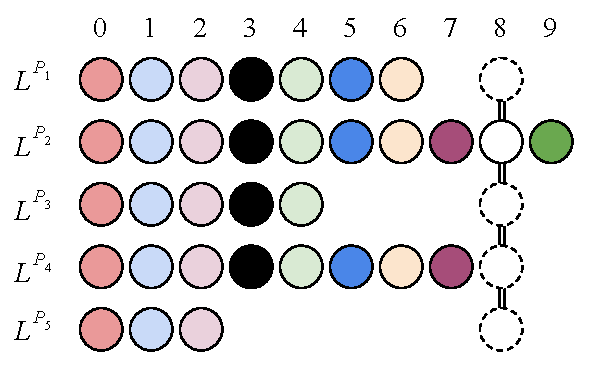
\includegraphics[width=0.65 \columnwidth,keepaspectratio]{figures/safe-ledgers.pdf}
    \caption{A god's eye view of the \emph{safe} ledgers of various honest parties at various moments in time.}
    \label{fig.safe-ledgers}
\end{figure}

Thinking back to the UTXO model, safety means that the transaction graph of one party is outdated, but not inconsistent, as compared
to the other party. In particular, if one party has confirmed a transaction $\tx$, then the other party cannot have confirmed, and can
never confirm, a transaction $\tx'$ which is a double spend of $\tx$. Let's try to understand why.

\begin{lemma}[Safe \Rightarrow No double spend (informal)]
In a safe protocol that ensures transaction validity locally,
two honest parties can never confirm two conflicting transactions.
\end{lemma}
\begin{proof}
Suppose, towards a contradiction, that party $P_1$ at time $r_1$ has confirmed $\tx$. This means that $\tx$ appears in $P_1$'s
ledger $L^{P_1}_{r_1}$ at time $r_1$, and let's call $i$ the position of the transaction in the ledger: $\tx = L^{P_1}_{r_1}[i]$.
Additionally, party $P_2$ at time $r_2$ has confirmed $\tx'$, a conflicting transaction to $\tx$. Similarly, let $j$ be the index:
$\tx' = L^{P_2}_{r_2}[j]$. Now, if $i = j$, then this means that $\tx = \tx'$, which is a contradiction since these are conflicting.
If $i < j$, then by safety this means that $L^{P_2}_{r_2}[i] = L^{P_1}_{r_1}[i] = \tx$. But then, party $P_2$ has included
in his ledger \emph{both} $\tx$ at position $i$ \emph{and} $\tx'$ at position $j$. This is a contradiction, because the honest
party validates $\tx'$ before accepting it. Therefore, the two parties cannot have accepted conflicting transactions.
\end{proof}

This is a good sanity check that our definition of safety makes sense. Is this revised and precise, yet weaker, notion of ledger
safety achieved by our \emph{longest chain} construction? Not quite. The problem is that, as we saw in the previous chapter,
the chain may have \emph{temporary forks} even when no adversary is mining. Whenever the chain \emph{reorgs}, there is a
potential for safety loss. Consider the case illustrated in Figure~\ref{fig:reorg-safety-loss}. Imagine that honest party
$P_1$ had initially adopted the chain whose tip is block $6$ and contains the top (green) transaction $\tx$. In the meantime
party $P_2$, who has not seen block $6$ yet, is still mining on top of block $4$. If party $P_2$ successfully mines block
$5$, he can include a double spending transaction in it, the bottom (red) transaction $\tx'$, conflicting with $\tx$.
Now the two chains at blocks $5$ and $6$ are at a tie. The tie will be broken when the next proof-
of-work is found (block $7$) and one branch becomes longer; the nodes that were working on the other
(block $6$) branch will then switch to the longer one. If we now compare the ledger reported by party $P_1$ when he
had adopted block $6$ and the ledger reported by party $P_2$ when he had block $7$, we see that the
ledgers obtained by \emph{reading} these two chains are mutually unsafe.

\begin{figure}[h]
    \centering
    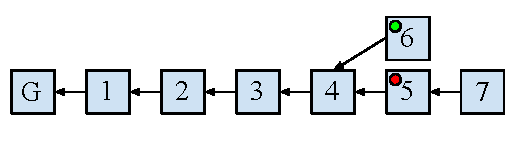
\includegraphics[width=0.65 \columnwidth,keepaspectratio]{figures/reorg-safety-loss.pdf}
    \caption{A chain reorg during a temporary fork causes a safety loss.}
    \label{fig.reorg-safety-loss}
\end{figure}

We will have to revise our \emph{reading rule} to account for these temporary forks. We now argue that these
temporary forks will be short. Let us initially analyze this claim in the setting where every miner is honest.
The idea is that, if we choose $T$ appropriately, then convergence opportunities will happen regularly.
Once a convergence opportunity happens, if there is no adversarial miner, the honest parties will converge into
one chain.

\begin{lemma}[Honest Convergence]\label{lem:honest-convergence}
    In a setting where only honest parties are mining, exactly $\Delta$ time after every convergence
    opportunity, all honest parties will hold the same chain.
\end{lemma}
\begin{proof}
    Consider an arbitrary convergence opportunity producing block $B$ occurring at time $r$.
    Since the convergence opportunity is $\Delta$ separated from every \emph{preceding} successful query,
    and all successful queries are honest and broadcast to the network, all honest parties will
    have seen all the blocks produced so far (because they all happen prior to $r - \Delta$ and it
    takes at most $\Delta$ time to receive the message containing those blocks).
    Therefore, the honest party who mined $B$
    will be mining on top of the longest chain among all. This means
    that, at time $r$, the block $B$ has a height larger than any other
    block. Because the miner is honest, he broadcasts $B$, and it is received by all honest parties within $\Delta$
    time. Since the convergence opportunity is $\Delta$ separated from every \emph{succeeding} successful
    query, no other blocks are mined or during the time interval $r \ldots r + \Delta$.
    At time $r + \Delta$, every honest party has received $B$ and adopted it since it is
    the longest chain. At this point, all the honest parties agree on their chains.
\end{proof}

\begin{itemize}
    \label{sec:liveness}
    \item \textbf{Liveness}: Honest transactions are included in all honest ledgers "soon".
\end{itemize}

\section{Chain Virtues}
\subsection{Virtues}
The liveness and safety of ledgers directly follow from chain virtues. For this reason, we outline fundamental properties that chains must uphold.
\begin{itemize}
    \item \textbf{Common Prefix($k$)}:
        Honest parties agree on their chains with the exception of the last $k$ blocks. This chain virtue will be used to prove ledger safety(\hyperref[sec:saftey]{Section 1}).
        \begin{figure}[h]
        \centering
        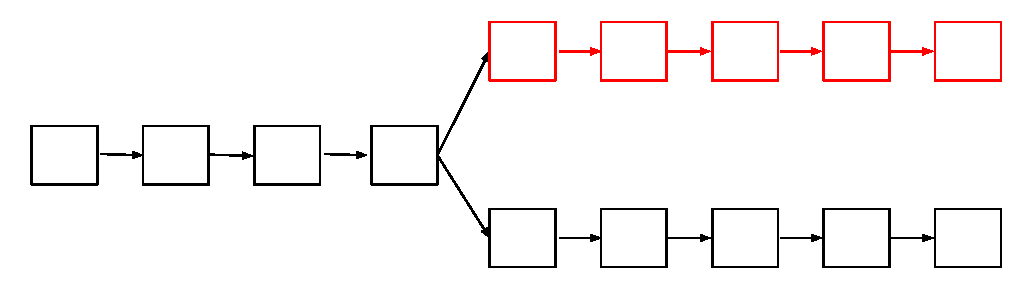
\includegraphics[width=\linewidth]{figures/commonprefix.pdf}
        \caption{These two chains satisfy the common prefix chain virtue with a $k$ of 6. The first 4 blocks of both chains are the honest parties common prefix.}
        \end{figure}
    \item \textbf{Chain Quality($\mu$)}: A sufficiently long chunk of the longest chain contains a $\mu > 0$ proportion of honest blocks.
    \begin{figure}[h]
    \centering
        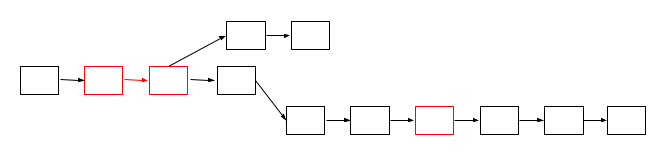
\includegraphics[width=\linewidth]{figures/chainquality.png}
        \caption{In this scenario the longest chain consists of 10 blocks. There are 3 blocks mined by an adversary and 7 honestly mined blocks in the longest chain. Hence, the chain quality $\mu$ of this chain is $70\%$. }
    \end{figure}
    \item \textbf{Chain Growth($\tau$)}: The chain adopted by honest parties will grow. Chain growth and chain quality will be used to prove the liveness virtue of ledgers(\hyperref[sec:liveness]{Section 1})

\end{itemize}

\subsection{Mechanics of Chain Divergence and Convergence}
Chain divergence happens when two or more blocks are mined at approximately the same time. When chain divergence happens, the honest node hash power is split up among multiple different chains. This is because there are multiple longest chains that the nodes can choose to extend. If blocks keep getting mined at the same time many chains can grow simultaneously. A convergence opportunity happens when exactly one block is mined with  period of silence of duration $\Delta$ before and after it. Honest parties move their hash power to extend the longest chain.
\begin{figure}
    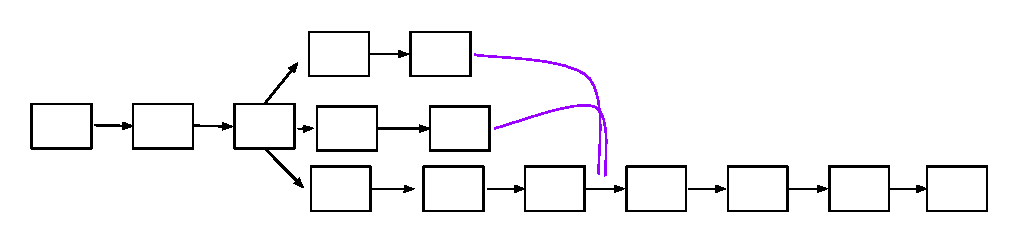
\includegraphics[width=\linewidth]{figures/divergence_convegence.pdf}
     \caption{In this scenario the chain diverges after the third block. This is because there were three blocks mined at about the same time. There is a convergence opportunity on the sixth block on the bottom chain. At this point honest nodes will switch over since they see the bottom chain is the new longest chain. The purple curved lines represent the honest parties switching over and adopting the new longest chain. }
    \label{sec:mechanics}
\end{figure}



\section{Network Attacks}
The attacks discussed in here are based on a strategy that gives rise to a "Nakamoto race".

Chain Quality is defined as the proportion of honestly mined blocks out of all mined blocks in a particular chain. A common conjecture is that Chain Quality can be approximated by the fraction of mining power that honest parties (however, future lectures will reveal that this is not the case).

In terms of chain virtues, the following attacks can break common prefix property and chain quality property if it were able to maintain the longest chain.

% Common prefix is broken if the adversary releases its chain to only a subset of nodes, thus making prefixes inconsistent until honest parties gossip amongst themselves. Chain quality is broken since a significant portion of the released chain is mined by the adversary.  Virtue \#2 (chain growth) is upheld as long as there are any honest participants mining that force the adversarial chain to grow.
\subsection{Nakamoto Attack}
The strategy of Nakamoto attack involves the adversary mining a competing chain in silent, withholding constituent blocks for as long as desired (often when the target adversarial transactions are buried $k$ blocks deep for instant confirmation). Therefore, since honest miners are unaware of that private adversarial chain, they continue extending the longest honest chain.
The adversary is, in effect, "racing" to construct a chain longer than the longest honest chain. If the private chain is longer that the honest chain, adversary can release the private chain. In such case, honest participants have to switch and extend the adversarial chain since it is the new longest chain. Thus, this adversarial chain replaces the honest chain. If the honest parties switch chains by reverting more than $k$ blocks, then the adversary has broken the Common Prefix property.

This attack is unlikely to succeed for a minority adversary. Consider the situation where the adversary and the honest parties begin mining at a particular block. Breaking Common Prefix requires that the honest parties mine a chain $k$ blocks long after that common block, while the adversary also mines $k$ or more blocks after the common block. As $k$ is chosen to be a somewhat large value, it will take time for the honest parties to mine $k$ blocks. Given that this span of time will be sufficiently large, the number of adversarially mined blocks will be fewer than the honest convergence opportunities within that timespan. If this is the case, the adversary cannot win.

\subsection{Fan-out Attack}
\begin{figure}
  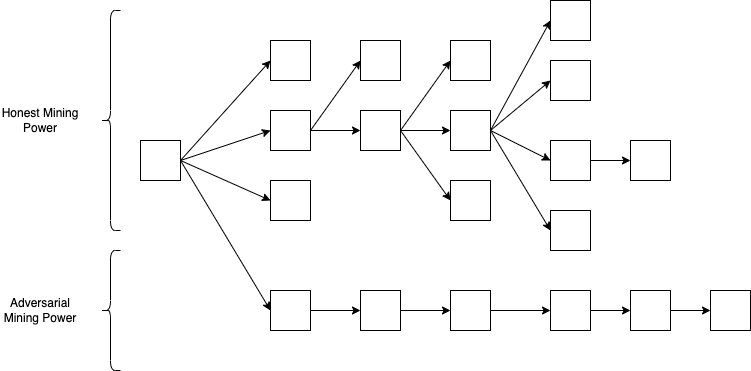
\includegraphics[width=\linewidth]{figures/fan_out.png}
  \caption{A fan-out attack where an adversary who does not hold majority hashing power can still produce the longest chain due to honest mining power being wasted. Displays a drawback of having infrequent convergence opportunities.}
  \label{fig:fan_out}
\end{figure}

This type of attack is unique in that it is more due to a fault of the network rather than an exploit from an adversary. Networks are susceptible to fan-out attacks when convergence opportunities are rare.

Infrequent convergence opportunities lead to honest nodes frequently working on competing chains, thus making the chain "fan out" as shown in \ref{fig:fan_out}. All but one of these competing branches are eventually thrown out, leading to the honest mining power being wasted. An adversary, on the other hand, can coordinate its attack to build on a single withheld chain, winning the race even without having majority hashing power. This is the reason why we do not want fast chains where the target is easily attainable.

\subsection{Majority Adversary Attack}
Now if the adversary held the majority of mining power in a network, all she needs to do is to mine a secret chain, which can be released at any time due to having more compute power. What properties can adversary break if she holds majority of the network hash power?

Clearly, she can violate the Common Prefix property as was mentioned earlier. If honest parties agree on the longest chain containing some block $B_m$, she mines a secret chain extending from the previous block $B_{m-1}$. Once the longest chain has $k$ or more blocks after $B_m$, she releases her secret chain to some of the honest miners. Since the adversarial chain is longer than the honest chain, these honest miners adopt the adversarial chain.

Additionally, an adversary with majority hash power can break Chain Quality as follows. If a block $B_m$ is mined by an honest miner, she creates a new longest chain extending the block $B_{m-1}$. Thus, the block $B_m$ is ``replaced" by a new block mined by the adversary. We will discuss this attack in more details in the next lecture.

However, in such attacks Chain Growth is upheld as long as there are any honest participants mining that force the adversarial chain to grow.
